\section{Preliminaries}

\begin{frame}\frametitle{Compressive Sensing 1/3}
Candes \& Donoho による信号や画像の低次元表現の枠組み
\begin{eqnarray}
    \inputSymbol & = & \dictSymbol \sparseSymbol, \;\;
    \dictSymbol \in \rsize{\inputSize \times \inputSize}
\end{eqnarray}
$\sparseSymbol$ 中で $\sparseness$ 個の係数しか大きな値を取らないとき,
$\sparseSymbol$ を $\inputSymbol$ の $\sparseness$ 疎表現と呼ぶ.
\begin{eqnarray}
    \featureSymbol & = & \rproSymbol \inputSymbol = \sensSymbol \sparseSymbol,
    \rproSymbol \in \rsize{\featureSize \times \inputSize} \\
    \sensSymbol & = & \rproSymbol \dictSymbol
\end{eqnarray}
上記の低次元空間への射影 $\sensSymbol$ を sensing matrix と呼ぶ.
\end{frame}


\begin{frame}\frametitle{Compressive Sensing 2/3}
疎表現の導出は $L_0$ ノルム(非零要素数)最適化問題
\begin{equation}
    \arg\min_{\sparseSymbol} ||\sparseSymbol||_0 \; s.t. \; \featureSymbol = \sensSymbol \sparseSymbol
\end{equation}
なので NP 困難だが,sensing matrix $\sensSymbol$ が
\begin{block}{Ristricted Isometry Property (RIP)}
$\mathbf{x}$ が任意の $K$ 疎ベクトルのとき
\begin{eqnarray}
    (1 - \delta) ||\mathbf{x}||^2_2 \leq & || \sensSymbol \mathbf{x} 
    ||^2_2 & \leq (1 + \delta) ||\mathbf{x}||^2_2 \\
    0 < & \delta & < 1
\end{eqnarray}
\end{block}
を満たすとき以下の$L1$ノルム最適化問題に近似できる\cite{Candes2008}.
\begin{equation}
    \arg\min_{\sparseSymbol}  ||\sparseSymbol||_1 \; s.t. \; \featureSymbol = \sensSymbol \sparseSymbol
\end{equation}
\end{frame}


\begin{frame}\frametitle{Compressive Sensing 3/3}
\begin{block}{主な$L_1$ノルム最適化アルゴリズム}
\begin{itemize}
    \item 貪欲法\\
        Match Pursuit (MP),
        Orthogonal MP (OMP)\footnote{筆者らは OMP を採用 (scikit-learn など多くのライブラリでも標準)}

    \item 凸緩和最適化\\
        Gradient Projection for Sparse Reconstruction (GPSR),\\
        Total Variation (TV),
        Smoothed-$L_0$ (S$L_0$)
\end{itemize}
\end{block}
\end{frame}


% \begin{frame}\frametitle{K-SVD の位置づけ}
% スパース表現の仲間 \cite{Murata2012}
% \end{frame}


\begin{frame}\frametitle{疎表現の問題設定}
\label{ksvd}
入力セット $\inputSymbol \in \rsize{\inputSize \times \datasetSize}$ に
最良の疎表現 $\sparseSymbol$ と辞書 $\dictSymbol$ は
$\mathbf{d}_{*,n}$ を $\dictSymbol$ の $n$ 列ベクトル,
$\mathbf{x}_{n,*}$ を $\sparseSymbol$ の $n$ 行ベクトルとすると
\begin{eqnarray}
    \min_{\dictSymbol, \sparseSymbol} ||\sparseSymbol||_0
    &s.t.& \min ||\inputSymbol-\dictSymbol\sparseSymbol||^2_2 \leq \varepsilon \\
    ||\inputSymbol-\dictSymbol\sparseSymbol||^2_F &=&
    ||\inputSymbol - \sum_{i} \mathbf{d}_{*,i} \mathbf{x}_{i,*}||^2_2 \\
    &=& ||(\inputSymbol - \sum_{i \neq n} \mathbf{d}_{*,i} \mathbf{x}_{i,*}) - \mathbf{d}_{*,n} \mathbf{x}_{n,*}||^2_2 \\
    &=& ||\mathbf{E}_n - \mathbf{d}_{*,n} \mathbf{x}_{n,*}||^2_2 \label{error}
\end{eqnarray}
式 (\ref{error}) を最小化する$\mathbf{d}_{*,n}, \mathbf{x}_{n,*}$ は
最小二乗法問題なので特異値分解(SVD)の解によって得られる
\footnote{http://www.misojiro.t.u-tokyo.ac.jp/~murota/lect-kisosuri/singularvalue050129.pdf}
\end{frame}


\begin{frame}\frametitle{K-SVD + OMP 更新アルゴリズム}
更新するのは $\dictSymbol, \sparseSymbol$ の2つ.適当に初期化しておく
\begin{algorithm}[H]
\begin{algorithmic}[1]
\FOR{$n=1$ to $N$}
%\COMMENT{疎表現 $n$ 次元目で非零のデータ番号集合}
\STATE $\Omega_n \leftarrow \{ i \in {1, \dots, I} | X_{n, i} \neq 0 \}$
\STATE $\mathbf{E}_n \leftarrow \{\inputSymbol_i\}_{i \in \Omega_n} - \sum_{i \in \Omega_n \setminus \{n\}} \mathbf{d}_{*,i} \mathbf{x}_{i,*}$
\STATE $\mathbf{U, S, V} \leftarrow \mathrm{SVD}(\mathbf{E}_n)$ \\
// 更新
\STATE $\mathbf{d}_{*,n} \leftarrow \mathbf{u}_{1,*}$
\STATE $\mathbf{x}_{n,*} \leftarrow s_{1,1} \mathbf{v}_{1,*}$
\ENDFOR
\end{algorithmic}
\caption{K-SVD + OMP}
\label{alg:seq}
\end{algorithm}
これを適当な回数反復する.OMPは収束が保証されている
\end{frame}


\begin{frame}{Singular Value Decomposition}
\begin{block}{特異値分解 (SVD)}
固有値分解を非正方行列に一般化

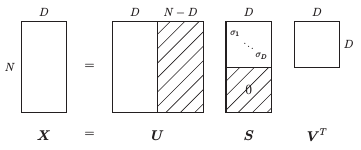
\includegraphics[height=2cm]{figure/svd.png}
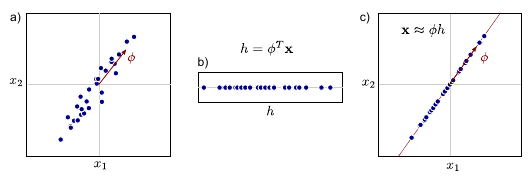
\includegraphics[height=2cm]{figure/svd1.png}

\begin{itemize}
    \item $U, V$ はユニタリ行列, 特異(列)ベクトルが並ぶ
    \item $S$ は非対角成分が零, 特異値が対角成分に並ぶ
    \item $(\cdot)^T$ は随伴 (複素共役かつ転置)
\end{itemize}
\end{block}
具体的な演算は省略\footnote{Lapackとかを使う}
\end{frame}


% \begin{frame}{Singular Value Decomposition 補足}
% \begin{block}{疑問}
% \begin{itemize}
%     \item なぜ特異値は分散と対応するのか
%     \item 第一列成分は分散(特異値)が最大となるのか
% \end{itemize}
% \end{block}
% \end{frame}


\begin{frame}\frametitle{Morphological image processing}
\begin{block}{Morphology}
特徴量抽出の前・後処理によく用いられる.主に以下の2種類
\begin{itemize}
    \item Dilation - 孤立点の除去
    \item Erosion - 欠落点の穴埋め
\end{itemize}
\end{block}

イメージ図\footnote
{\url{http://jp.mathworks.com/help/images/morphology-fundamentals-dilation-and-erosion.html}}
:実際は円状の構造要素(図中灰色)を利用
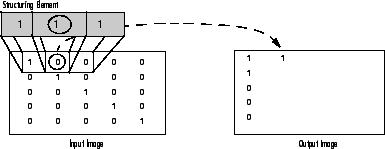
\includegraphics[scale=0.4]{figure/morph.png}
\end{frame}
